\subsubsubsection{Bootstrap}
The bootstrap process consists of two ordered parts:
\begin{enumerate}
	\item \textit{Initialization} - instantiates and configures the necessary resources for the application;
	\item \textit{Activation} - starts the application.
\end{enumerate}
Clearly, activation depends on initialization.
While the initialization process is automatically triggered at node
creation, this is not the case for activation which is triggered by
the middleware.
Moreover, at Application Layer level, we have to consider the
dependencies among the entity types exposed in \ref{fig:sd-entity-types-deps}.
The overall bootstrap process, which mimics UNIX init
\footnote{http://www.tldp.org/LDP/sag/html/index.html},
is divided in two ordered parts:
\begin{enumerate}
	\item \textit{Init} - initialize all the sub-layers of each macro layer
	following a bottom up approach (from \verb|interface_layer.session| to
	\verb|application.scheduling|).
	The initialization order is given by the fact that the upper
	layers need the services provided by the underlying layers to work
	correctly (Figure \ref{fig:sd-app-init});
	\item \textit{start} - the first tick forwarded from the middleware to the
	Application Layer through Interface Layer. As stated, this event is
	exclusively triggered by the middleware.
\end{enumerate}
\begin{figure}[H]
  \centering
  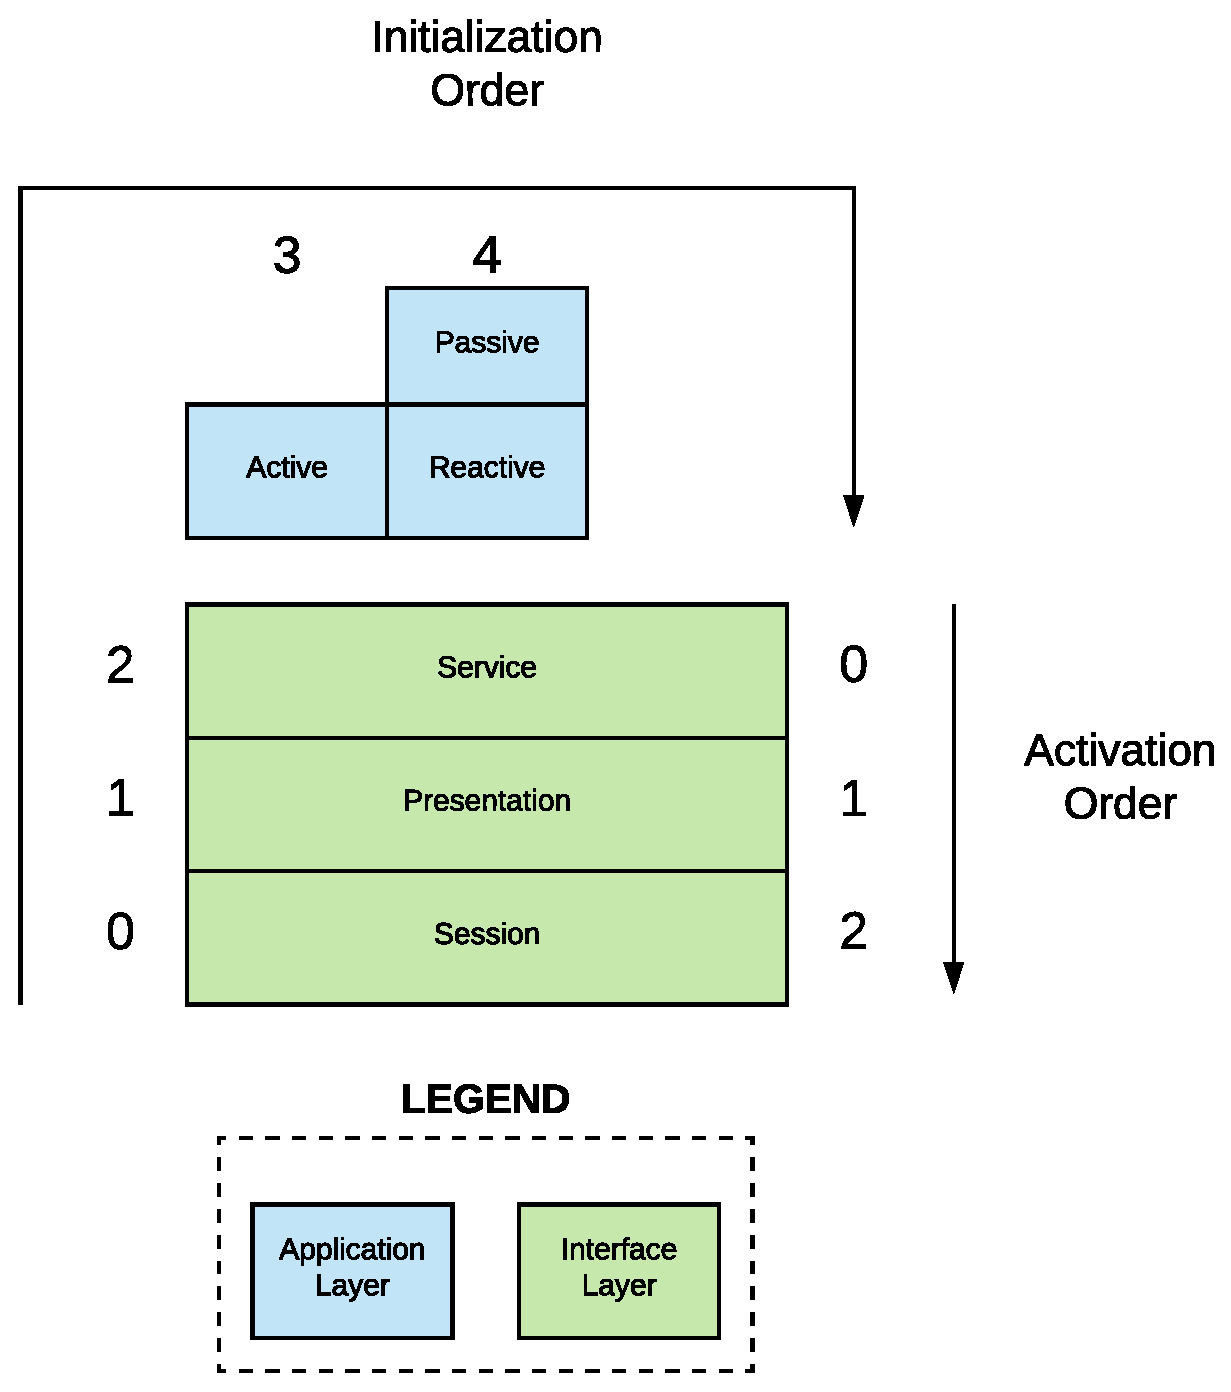
\includegraphics[scale=0.5,keepaspectratio]
    {images/solution/init_activate.eps}
  \caption{Application Bootstrap - Init}
  \label{fig:sd-app-init}
\end{figure}


\subsubsubsubsection{Init}

Each application node contains the \textit{Init} process,
which is the parent of all the application processes.
The execution steps of \textit{Init} are depicted in Figure
\ref{fig:sd-app-init}.
It instantiates the resources of each layer, thus making
Interface Layer and Application Layer transit from \verb|inactive|
to \verb|ready| state.
For example, each sub-layer of Interface Layer instantiate its own pool of
LWPs\footnote{light weight processes}.
\\
The Application Layer initialization completes in the following order:
\begin{enumerate}
	\item \textit{Active} - the entities which moves in the city
	(e.g. pedestrians);
	\item \textit{Reactive} - the infrastructure of the city (e.g. district);
	\item \textit{Scheduling} - the sub-layer which handles the execution order
	and generates synchronization signals for the events of Application Layer.
\end{enumerate}
Note that the \textit{Passive} entities have no particular dependency. Since
they are stateless and they logically belong to \textit{reactive} entities
(e.g. road signs belong to roads), they will be instantiated along with them.
When the scheduling sub-layer completes its initialization, init signals
the application layer completion to each sub-layer of Interface Layer in the
following order:
\begin{enumerate}
	\item \textit{Service} - provides activators and pipelines services to
	application layer;
	\item \textit{Presentation} - provides data conversion services;
	\item \textit{Session} - provides network connection services
	(e.g. sender, receiver).
\end{enumerate}
Init triggers the switch of each Interface sub-layer state from
\verb|ready| to \verb|active|.
The activation order is extremely important to
proactively avoid the lost of messages between remote nodes. Indeed, at this
stage, the application layer is not able to generate or receive messages
because the start message has not been sent by the middleware.
The service and
the presentation layer are activated before the session layer; the latter
exposes a remote communication channel (a connection to a TCP socket).
Finally, the application is ready to communicate because each of its layers
has been activated. Now, the Application waits the \verb|start| tick from the
middleware.

A crash of the \textit{Init} process, occurring before the end of the bootstrap,
is signaled to the middleware layer, by the expiration of a timeout from the
middleware side.
Note that this model works also for a bootstrap which is executed starting
from a snapshot of the system, with the only difference consisting in divergent
values of the configuration file. Indeed, we have to use a set of
configurations, which is going to be different for each city.

\subsubsubsubsection{Start}

When \textit{Init} completes, the Application Layer is in a \verb|ready| state
while Interface Layer is in an \verb|active| state.
The first message sent by the middleware towards the
Interface Layer will be a \verb|start| message,
which will trigger the Application Layer activation.
The \verb|start| message will be converted into a scheduler
\verb|tick| which will enable the latter to consume the first work item
(i.e. a list of registered agents actions) of its agenda.